\subsection{Photoframe identification}
\label{sse:ident_photoframe}

\noindent The photoframe identification module performs the identification of textured model images with a black frame around the texture as shown in Figure~\ref{fig:ident_photoframe}. 

\begin{figure}[H]
\centering
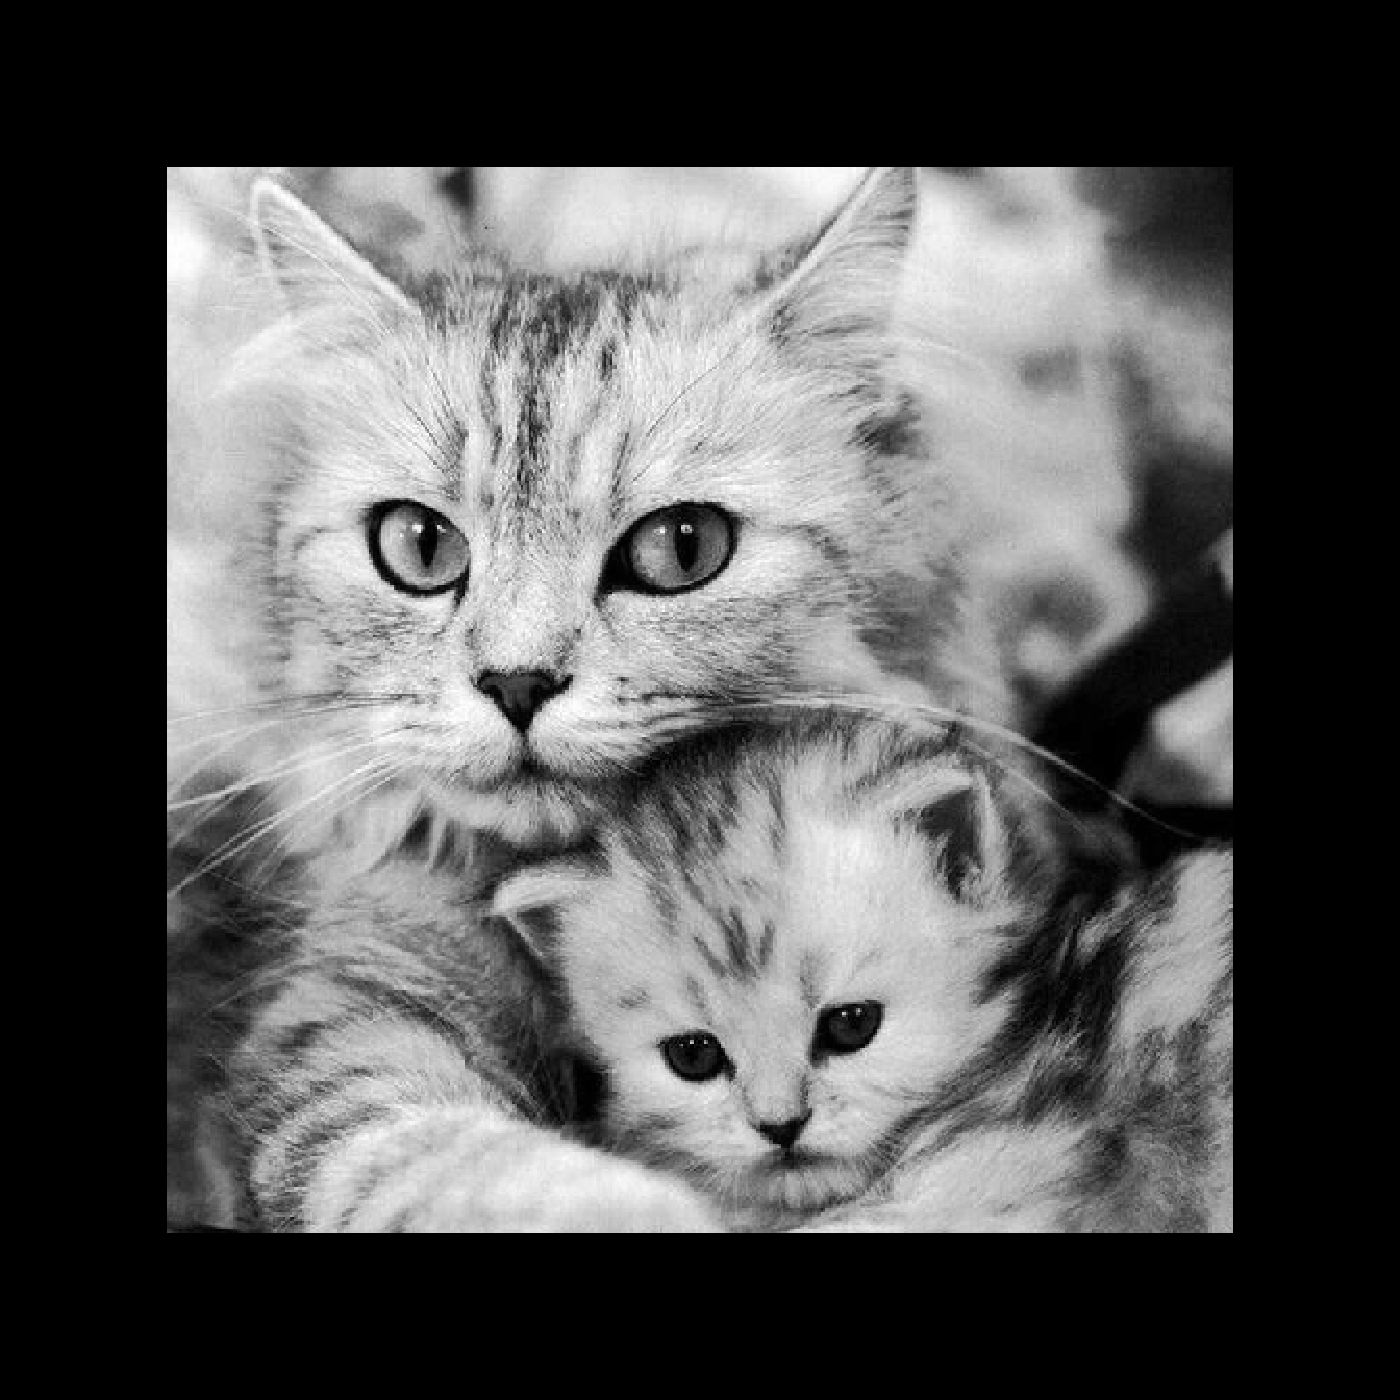
\includegraphics[width=0.45\textwidth]{vision/figures/ident_photoframe} 
\caption{Examples of model that can be identified with the photoframe identification module.}
\label{fig:ident_photoframe}
\end{figure}

The photoframe image model identification is faster than the
identification of phototexture image model since the identification
take benefit of the detection of the black frame around the texture.
On the other hand, the black frame shall be fully visible in the image.

\subsubsection{The {\tt Rox\_Ident\_Photoframe\_SE3} object}
\label{sss:ident_photoframe_object}
A \lstinline$Rox_Ident_Photoframe_SE3$ object is a pointer to the opaque structure \lstinline$Rox_Ident_Photoframe_SE3_Struct$: 

\begin{lstlisting}
typedef struct Rox_Ident_Photoframe_SE3_Struct * Rox_Ident_Photoframe_SE3
\end{lstlisting}

\subsubsection{Creating/Deleting a {\tt Rox\_Ident\_Photoframe\_SE3}}
\label{sss:ident_photoframe_newdel}
~\\

\noindent The rox\_ident\_photoframe object shall be created before any call to other functions using it :

\begin{lstlisting}
Rox_Error rox_ident_photoframe_new(Rox_Ident_Photoframe * ident_photoframe) 
\end{lstlisting}

\noindent This function creates a new empty database object.

\begin{lstlisting}
Rox_Error rox_ident_photoframe_del(Rox_Ident_Photoframe * ident_photoframe)
\end{lstlisting}


\subsubsection{Main functions related to {\tt Rox\_Ident\_Photoframe\_SE3}}
\label{sss:ident_photoframe_functions}
~\\

\noindent A photoframe is a planar object specifically designed to be identified
when filmed with a camera. It is a composition of an image template, a
thick black border and a white background outside of the border.
Figure 1 explains the common scheme of a photoframe.  The image inside
the black borders is the \emph{template}. This template is the object
to identify, and which will be used to track the object after
detection if needed. This template size is
$\left[image \; rows, image \; cols\right]$.  Values iheight and iwidth shall be
equal to 128 pixels.

\begin{figure}[h]
\centering{}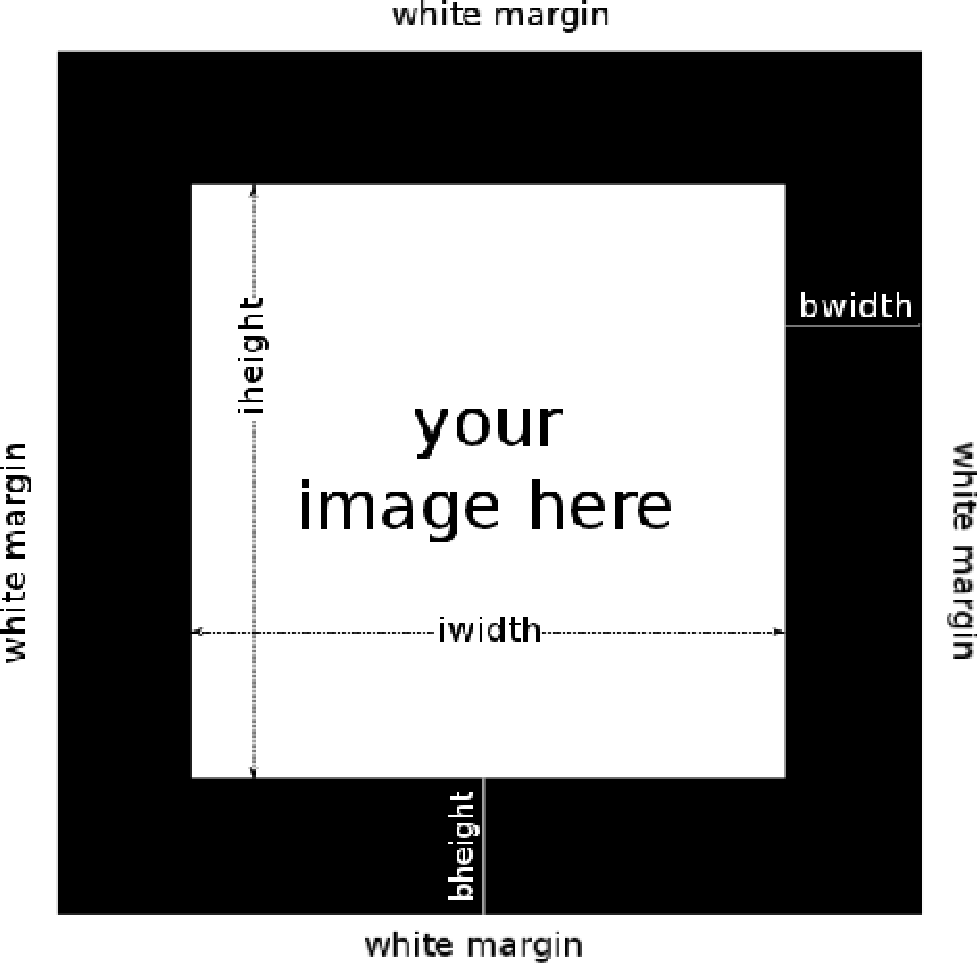
\includegraphics[width=0.6\columnwidth]{vision/figures/fake}
\caption{A common photoframe scheme}
\end{figure}

\noindent The border size $\left[border \; rows, border \;
  cols\right]$ is choosed optimally to be visible in a large set of
viewpoints while not being too large (i.e. not wasting image space).
The following calculus is done to compute border size :

\begin{itemize}
\item border rows = $\frac{80}{512}$ image rows
\item border cols = $\frac{80}{512}$ image cols
\end{itemize}

\noindent Be sure to respect those sizes when creating your photoframe or the
identification performance will be severely degraded.\\

\noindent To create a photoframe, choose a template image which is compatible
with \rox{} (non uniform, with enough texture). Store this template in
a PGM image file. With an image editing software (E.g. : photoshop,
gimp) draw the borders in black color (See figure 1). Print this image
on a white paper sheet. Because of printers approximation, it is not
possible to know what will be the exact size (in meters) of this
print.  Take a ruler to measure the width and height of the image
template \emph{inside} the black borders. These real sizes are only
needed if used to compute odometry after identification. Repeat this
operation for each photoframe you need.\\

\noindent The user can go through the following workflow:

\begin{enumerate}
\item An identification structure is created (see section~\ref{sss:ident_photoframe_newdel}).
\item Template images are added to the identification module using the following function:

\begin{lstlisting}
Rox_Error 	rox_ident_photoframe_se3_addframe (Rox_Ident_PhotoFrame_SE3 obj, Rox_Image model, Rox_Real width_meter, Rox_Real height_meter, Rox_Uint border_width);
\end{lstlisting}

\noindent Adds a new template to a photoframe identification
structure. Shall be called before identification. First parameter is a
pointer created with rox\_ident\_new, second parameter is the template
image to add (without black borders) with a size of 128x128 pixels.
Please note that one photoframe will be identified only once in one
image. If several instances of the same photoframe are in the
processed image, only the first found will be considered. Note that
the identifier of the added photoframe will be the number of times
this function has already been called.

\item The user grabs an image from a stream (e.g. a camera) and gives it
  to photoframe identification. The identification is done and the
  number of identified templates are stored in the \lstinline $Rox_Ident_PhotoFrame_SE3$ object:

\begin{lstlisting}
Rox_Error rox_ident_photoframe_se3_make (Rox_Ident_PhotoFrame_SE3 obj, Rox_Camera camera);
\end{lstlisting}

\noindent Using the ident structure created with rox\_ident\_new and filled
with templates using rox\_ident\_add\_photoframe, tries to detect
photoframes in the given image. This image may be given by a camera
for example. Returns the number of identified photoframes in the current
image.

\item For each template, the user can check if it has been identified using the following function:

\begin{lstlisting}
Rox_Error rox_ident_photoframe_se3_getresult (Rox_Uint *is_identified, Rox_MatSE3 pose, Rox_Ident_PhotoFrame_SE3 obj, Rox_Uint id);
\end{lstlisting}

\noindent Used after a call to rox\_ident\_photoframe. Checks if a given photoframe
(using its id) has been detected or not. ident is a
pointer to a photoframe identification structure created with rox\_ident\_new.
photoframe\_id is a number between 0 and the number of added frames.
Returns Rox\_True if the specific photoframe is detected, Rox\_False
otherwise.

% \item If the template is identified, a function returns a 2D transformation which
% measures how the template is ``seen'' in the current grabbed image.

% \begin{lstlisting}
% Rox_MatSL3 rox_ident_photoframe_get_matsl3(Rox_Ident ident, Rox_Uint id);
% \end{lstlisting}

\noindent Used after a call to rox\_ident\_photoframe and rox\_ident\_get\_identified.
If a photoframe with id has been identified, returns the 2D
transformation which represents the template image (without the borders)
in the current image. 2D transformation is not defined (and may contain
random value) if the marker is not identified.\\

\item Once not used anymore, the identification structure shall
be deleted (see section~\ref{sss:ident_photoframe_newdel}).
\end{enumerate}
